\documentclass[12pt,a4paper]{article}
\usepackage{rmpackages}																% usual packages
\usepackage{rmtemplate}																% graphic charter
\usepackage{rmexocptce}																% for DS with cptce eval

\cfoot{} 														% if no page number is needed
%\renewcommand\arraystretch{1.5}		% stretch table line height

\begin{document}

\begin{header}
	Les défis confinés -- Épisode 8
\end{header}

\begin{center}
	\color{red}
	\begin{bfseries}
		\warning{} \warning{} \warning{}
		Ne JAMAIS regarder directement le Soleil !
		\warning{} \warning{} \warning{}
	\end{bfseries}
		
	Sa lumière est trop intense : elle peut endommager de manière irréversible votre vision.
	
	Ceci est également valable pour le spectroscope et, de manière générale, pour tout dispositif optique non exclusivement prévu à cet effet !
\end{center}

\section*{Un spectroscope maison}

\begin{multicols}{2}
	Comme vous l'avez vu la semaine dernière, on peut obtenir le spectre d'un rayonnement avec un élément dispersif : un prisme ou mieux, un \textbf{réseau}.
	Un réseau est composé d'une série de fentes ou de rayures espacées de façon régulière : exactement comme un CD.
	C'est pour cela que les disques présentent des réflexions colorées.
	
	Grâce à un CD, on peut ainsi fabriquer un spectroscope qui permettra d'analyser la lumière issue de sources différentes.
	\vfill

	\begin{center}
		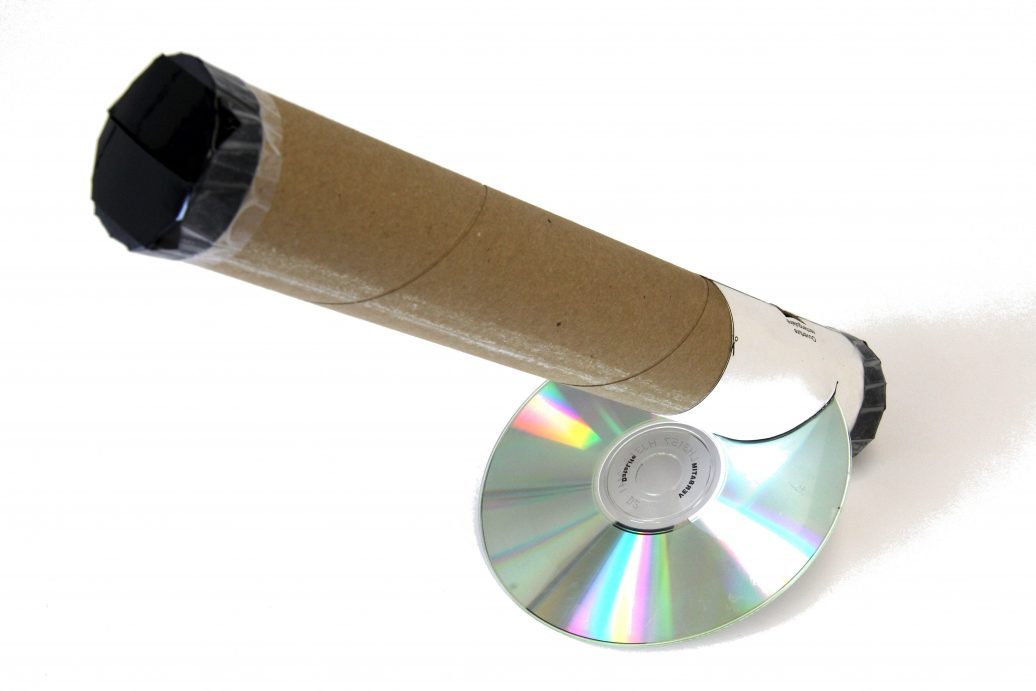
\includegraphics[width=\linewidth]{images/spectro.jpg}
	\end{center}
\end{multicols}

Le lien ci-dessous vous mènera vers un mode d'emploi pour fabriquer votre spectroscope.
Une vidéo vous montrera aussi comment le réaliser.
Vous posterez une photo de votre spectroscope et de vos observations, en précisant de quelle source de lumière il s'agit, sur la conversation Teams dédiée.

\begin{center}
\href{https://www.cdsp.qc.ca/conference/empreintes-lumineuses/lumiere-experience-maison/}{https://www.cdsp.qc.ca/conference/empreintes-lumineuses/lumiere-experience-maison/}
\end{center}

\paragraph*{Conseils}
\begin{itemize}
	\item[•] Le mode d'emploi propose d'utiliser un guide de coupe à imprimer.
	Si vous n'avez pas d'imprimante, il suffit de réaliser l'incision dans le tube de telle sorte que le CD soit incliné à environ \SI{60}{\degree} par rapport au tube.
	\item[•] Certains disques produisent de meilleurs résultats que d'autres : essayez avec un CD, un DVD, etc. pour choisir celui qui fonctionne le mieux.
	\item[•] Pour obtenir de jolis spectres, il faut que la lumière entre uniquement par la fente : utilisez du ruban adhésif opaque pour boucher toutes les autres ouvertures, ou de la feuille d'aluminium.
	\item[•] Attention avec le cutter : ne vous coupez pas !
\end{itemize}

\end{document}

\href{http://toysfab.com/2018/03/fabriquer-un-spectrometre-avec-votre-smartphone/}{http://toysfab.com/2018/03/fabriquer-un-spectrometre-avec-votre-smartphone/}